\documentclass[11pt,twoside,a4paper]{article}
% http://www-h.eng.cam.ac.uk/help/tpl/textprocessing/latex_maths+pix/node6.html symboles de math
% http://fr.wikibooks.org/wiki/Programmation_LaTeX Programmation latex (wikibook)
%=========================== En-Tete =================================
%--- Insertion de paquetages (optionnel) ---
\usepackage[french]{babel}   % pour dire que le texte est en fran{\'e}ais
\usepackage{a4}	             % pour la taille   
\usepackage[T1]{fontenc}     % pour les font postscript
\usepackage{epsfig}          % pour gerer les images
%\usepackage{psfig}
\usepackage{amsmath, amsthm} % tres bon mode mathematique
\usepackage{amsfonts,amssymb}% permet la definition des ensembles
\usepackage{float}           % pour le placement des figure
\usepackage{verbatim}

\usepackage{longtable} % pour les tableaux de plusieurs pages

\usepackage[table]{xcolor} % couleur de fond des cellules de tableaux

\usepackage{lastpage}

\usepackage{multirow}

\usepackage{multicol} % pour {\'e}crire dans certaines zones en colonnes : \begin{multicols}{nb colonnes}...\end{multicols} 

% \usepackage[top=1.5cm, bottom=1.5cm, left=1.5cm, right=1.5cm]{geometry}
% gauche, haut, droite, bas, entete, ente2txt, pied, txt2pied
\usepackage{vmargin}
\setmarginsrb{1.00cm}{1.00cm}{1.00cm}{1.00cm}{15pt}{3pt}{50pt}{20pt}

\usepackage{lscape} % changement orientation page
%\usepackage{frbib} % enlever pour obtenir references en anglais
% --- style de page (pour les en-tete) ---
\pagestyle{empty}

\def\txtTITLE{Grandeur Nature, Aspect L{\'e}gal} %%%%% !! TITRE !! %%%%%
\def\imgCORNER{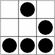
\includegraphics[width=0.25cm]{../../../../../imgGraphics/logos/glider/logo-glider.png}}

%--- Definitions de nouvelles couleurs ---
\definecolor{verylightgrey}{rgb}{0.8,0.8,0.8}
\definecolor{verylightgray}{gray}{0.80}
\definecolor{lightgrey}{rgb}{0.6,0.6,0.6}
\definecolor{lightgray}{gray}{0.6}

% % % en-tete et pieds de page configurables : fancyhdr.sty

% http://www.trustonme.net/didactels/250.html

% http://ww3.ac-poitiers.fr/math/tex/pratique/entete/entete.htm
% http://www.ctan.org/tex-archive/macros/latex/contrib/fancyhdr/fancyhdr.pdf
%% \usepackage{fancyhdr}
%% \pagestyle{fancy}
%% % \newcommand{\chaptermark}[1]{\markboth{#1}{}}
%% % \newcommand{\sectionmark}[1]{\markright{\thesection\ #1}}
%% \fancyhf{}
%% \fancyhead[LE,RO]{\bfseries\thepage}
%% \fancyhead[LO]{\bfseries\rightmark}
%% \fancyhead[RE]{\bfseries\leftmark}
%% \fancyfoot[LE]{\thepage /\pageref{LastPage} \hfill
%% 	\scriptsize{\txtTITLE} % TITLE
%% \hfill \imgCORNER }
%% \fancyfoot[RO]{\imgCORNER \hfill
%% 	\scriptsize{\txtTITLE} % TITLE
%% \hfill \thepage /\pageref{LastPage}}
%% \renewcommand{\headrulewidth}{0.5pt}
%% \renewcommand{\footrulewidth}{0.5pt}
%% \addtolength{\headheight}{0.5pt}
%% % \fancypagestyle{plain}{
%% 	% \fancyhead{}
%% 	% \renewcommand{\headrulewidth}{0pt}
%% % }

\usepackage{lettrine}
\usepackage{fancybox}

\title{\txtTITLE}
\date{ --- }

%============================= Corps =================================
\begin{document}

\setlength\parindent{0pt} % \noindent for all document

\begin{center}
	\textbf{\huge \txtTITLE}
\end{center}

%% \textbf{\Large L'aspect l{\'e}gal}~\\

\textbf{\scriptsize Le jeu de r{\^o}le grandeur nature a beau {\^e}tre un loisir, il ne se pratique pas sans quelques pr{\'e}cautions et autorisations. Pas question en effet de d{\'e}barquer en bande costum{\'e}e dans une for{\^e}t sans en avoir auparavant demand{\'e} la permission. } %% ~\\
\texttt{\scriptsize{(Originellement Publi{\'e} dans : Casus Belli Hors s{\'e}rie n 4 -- Le Jeu de R{\^o}le Grandeur Nature (GN), 1992 -- Excelsior Publications)}}~\\

\begin{multicols*}{2}
	%% \small

\textbf{\large Les autorisations}~\\

Dans la plupart des cas de figure, vous aurez besoin d'autorisations pour l'organisation d'un jeu de r{\^o}le grandeur nature. Contactez les gens par t{\'e}l{\'e}phone ou par courrier, et demandez un rendez-vous (le jour de la reconnaissance). Il vaut peut-{\^e}tre mieux s'expliquer directement, et vous pourrez ainsi fournir tous les renseignements utiles. Si votre courrier n'a pas de r{\'e}ponse, insistez par t{\'e}l{\'e}phone. ~\\

\textbf{\textit{\large En for{\^e}t}}~\\

Pour savoir de qui d{\'e}pend une zone de for{\^e}t que vous avez choisie (domaniale, priv{\'e}e, r{\'e}serve de chasse...), contactez la mairie la plus proche. --- S'il s'agit d'une for{\^e}t domaniale contactez l'Office National des eaux et For{\^e}ts (ONF) et la gendarmerie. ~\\

Cherchez l'adresse de la maison foresti{\`e}re dont d{\'e}pend votre zone de jeu, pour joindre la personne responsable (un d{\'e}tail au passage : le terme << garde forestier >> ne s'utilise plus et n'est g{\'e}n{\'e}ralement pas tr{\`e}s appr{\'e}ci{\'e}. Le responsable est souvent un ing{\'e}nieur...). Demandez par {\'e}crit l'autorisation d'organiser un jeu de r{\^o}les grandeur nature dans la r{\'e}gion. Joignez une copie de la carte IGN o{\`u} vous aurez indiqu{\'e} les limites de votre aire de jeu. Si votre interlocuteur ne sait pas ce qu'est un jeu de r{\^o}le grandeur nature, expliquez-lui en termes simples ou en l'assimilant  {\'e}ventuellement {\`a} un rallye, un jeu de piste ou une reconstitution historique. ~\\

L'ONF vous indiquera les endroits o{\`u} il est interdit de se rendre (r{\'e}serves naturelles, par exemple), les interdits (comme le feu !) et autres consignes de s{\'e}curit{\'e}. ~\\

Pr{\'e}venez aussi la gendarmerie. Elle effectue souvent des rondes et risque d'{\^e}tre surprise par les activit{\'e}s nocturnes d'une centaine de personnes en costume m{\'e}di{\'e}val ! ~\\

Pour le camping, si vous avez pr{\'e}vu un h{\'e}bergement sous tente, sachez qu'il est g{\'e}n{\'e}ralement interdit en France dans les for{\^e}ts domaniales. Trouvez un accord avec l'agent de l'ONF ou cherchez le pr{\'e} le plus proche et renseignez-vous sur son propri{\'e}taire. Il est rare qu'un agriculteur vous refuse l'autorisation de camper sur un pr{\'e} inoccup{\'e}. ~\\

\textbf{\textit{\large En ville, dans les rues}}~\\

Contactez la mairie pour les autorisations et le commissariat (ou la gendarmerie). Ce dernier ne vous d{\'e}livrera pas d'autorisation {\`a} proprement parler, mais il vaut mieux mettre la Police au courant de votre manifestation. Surtout si vous organisez un jeu contemporain mettant en sc{\`e}ne des espions qui se poursuivent dans les rues avec un pistolet {\`a} la main ! On a malheureusement en m{\'e}moire la m{\'e}saventure de plusieurs joueurs qui ont pass{\'e}s une nuit au poste car les organisateurs, peu consciencieux, avaient omis de pr{\'e}venir le commissariat qu'ils organisaient un jeu d'espionnage dans leur quartier... ~\\

\textbf{\textit{\large Dans une propri{\'e}t{\'e} priv{\'e}e}}~\\

G{\'e}n{\'e}ralement aucune autorisation n'est n{\'e}cessaire. Les lieux priv{\'e}s comprennent les centres culturels, les centres de vacances, les salles des f{\^e}tes municipales, certaines parcelles de for{\^e}ts, les sites lou{\'e}s, etc. ~\\

Cependant, renseignez-vous sur les d{\'e}crets municipaux. Il se peut qu'il soit impossible, par exemple, de faire du bruit apr{\`e}s 21 heures ou que la circulation soit interdite aux v{\'e}hicules {\`a} moteurs dans certains quartiers {\`a} des dates pr{\'e}cises (f{\^e}tes, march{\'e}s). %% ~\\

\begin{center} \rule{0.45\textwidth}{0.01cm} \end{center}

Demandez toujours les autorisations qui vous seront n{\'e}cessaires par {\'e}crit, et demandez aussi un accord {\'e}crit. En cas de probl{\`e}me, ces documents seront indispensables. Il arrive en effet que l'information circule mal et que, par exemple, un conseiller municipal se m{\^e}le, le jour m{\^e}me du jeu, de vous interdire l'acc{\`e}s au terrain de camping de la commune. Si  vous pouvez lui montrer une lettre {\`a} en-t{\^e}te de la mairie vous autorisant {\`a} monter vos tentes, vous {\'e}viterez un longue heure d'explications houleuses... ~\\

Pr{\'e}venez aussi gentiment les voisins des lieux o{\`u} se d{\'e}roulera le jeu. Excusez-vous {\`a} l'avance du bruit que pourront faire les participants et expliquez-leur au mieux la situation. N'envoyez pas de courrier, qui est trop impersonnel, mais rendez-leur visite. ~\\

\vfill
\clearpage

\textbf{\large L'assurance}~\\

Elle est indispensable. En tant qu'organisateur, votre responsabilit{\'e} civile est engag{\'e}e sur un certain nombre de points. Si un {\'e}l{\'e}ment de d{\'e}cor {\'e}crase le capot d'une voiture, si le saucisson du banquet provoque une intoxication alimentaire ou si votre fumig{\`e}ne met le feu {\`a} une for{\^e}t, vous serez l{\'e}galement responsable. Un contrat de responsabilit{\'e} civile pour l'organisation d'une manifestation couvre les dommages (corporels ou aux biens) pouvant {\^e}tre caus{\'e}s involontairement {\`a} autrui. Attention, la responsabilit{\'e} de l'organisateur doit {\^e}tre clairement mise en cause pour que l'assurance intervienne. ~\\

Par contre, si un joueur en blesse un autre, s'il renverse un pot de fleur sur la t{\^e}te d'un passant ou s'il se casse le bras en sautant d'un arbre, c'est sa propre responsabilit{\'e} qui est engag{\'e}e et il ne pourra pas se retourner contre vous. C'st pour cette raison que les participants doivent signer une d{\'e}charge sur leur feuille d'inscription. ~\\

N'oubliez pas que les compagnies d'assurance vous demanderont de satisfaire {\`a} certains crit{\`e}res pour vous couvrir. Par exemple, les endroits dangereux doivent {\^e}tre nettement balis{\'e}s. Renseignez-vous sur les limites de votre contrat et sur les conditions que vous devez satisfaire. Attention, d{\`e}s que vous utilisez des effets sp{\'e}ciaux mettant en jeu du feu, le co{\^u}t de l'assurance risque de grimper d'une fa\c{c}on spectaculaire. ~\\

Actuellement, il semble que les compagnies d'assurances proposent deux types de contrat [1985-1990] : 
\begin{itemize}
	\item[$\bullet$] \textbf{Un forfait pour une seule manifestation. }Pour vous donner un ordre d'id{\'e}e, il faut compter entre 300 et 400 francs pour un week-end de 100 personnes. 
	\item[$\bullet$] \textbf{Une cotisation annuelle, quelque soit le nombre de manifestations organis{\'e}es. }Il faut souvent ajouter au prix de base (dans les 400 francs), un forfait par membre de l'association (30 {\`a} 50 francs), plus une assurance compl{\'e}mentaire par jour et par participant (0,50 {\`a} 1 franc). Cette formule n'est interessante que si vous organisez un certain nombre de manifestations par an. 
\end{itemize}

Attention, ces prix ne sont donn{\'e}s qu'{\`a} titre indicatif. Renseignez-vous aupr{\`e}s de plusieurs compagnies, faites jouer la concurrence et ne vous adressez pas forc{\'e}ment aux plus grosses soci{\'e}t{\'e}s. Un courtier ou une petite compagnie proposent quelquefois des tarifs bien plus avantageux. ~\\

Vous pouvez aussi pr{\'e}voir une assurance << assistance m{\'e}dicale rapatriement >> (style \emph{Europ-Assistance}), mais elle n'est pas obligatoire du point de vue l{\'e}gal. Elle peut n{\'e}anmoins se r{\'e}v{\'e}ler tr{\`e}s pratique si vous organisez un jeu d'une semaine dans le Vercors, par exemple. ~\\

\end{multicols*}

\end{document}
